\documentclass[a4paper,12pt,twoside]{article}

% ----- Header ----- %
\title{FPGA Development for the LHCb Vertex Locator Upgrade}
\author
{
	Nicholas Mead\\
	Student Number: 8064141\\
	School of Physics and Astronomy\\
	University of Manchester
}
\date{\today}

% ----- Packages ----- %
\usepackage[left=1in,right=1in,bottom=1.25in,top=1in]{geometry}
\usepackage{amsmath}
\numberwithin{equation}{section}
\numberwithin{figure}{section}
\numberwithin{table}{section}
\usepackage{graphicx}
\graphicspath{{Figures/}}
\usepackage{amsfonts}
\usepackage{bm}
\usepackage{enumerate}
\usepackage[ampersand]{easylist}
\usepackage{lineno}
\usepackage[backend=biber,sorting=none]{biblatex}
\addbibresource{Report_Main.bib}
\usepackage{placeins}
\let\Oldsection\section
\renewcommand{\section}{\FloatBarrier\Oldsection}
\let\Oldsubsection\subsection
\renewcommand{\subsection}{\FloatBarrier\Oldsubsection}
\let\Oldsubsubsection\subsubsection
\renewcommand{\subsubsection}{\FloatBarrier\Oldsubsubsection}
\usepackage{hhline} %double line for table
\usepackage{arydshln}
\let\hdash\hdashline
\usepackage[thinlines]{easytable}
\usepackage[font=footnotesize,labelfont=bf]{caption} %figure captions
\usepackage{sidecap} %side captions
\sidecaptionvpos{figure}{c}

% ----- Settings ----- %	
\setlength{\parindent}{0em}
\setlength{\parskip}{1em}

% ----- Main ----- %
\begin{document}

	% ----- Document Head ----- %
	\begin{titlepage}
		\clearpage
		\maketitle \thispagestyle{empty}
		\vspace{1em}
		\begin{abstract}
	\hspace{-2em}
	This document discusses two areas of FPGA development for the LHCb VELO upgrade scheduled to coincide with LHC Long Shutdown 2 in 2019.
	The areas of development are the selection of a suitable scrambling algorithum and the continued work on the event isolation flagging.
	\\ \\
	The analaysis for three scrambling algorithms, required for data transfer from the front end elctronics to the Data Aquisition FPGA, was compared against the theoretical predictions of scrambled data.
	It was found that the currently implemented VeloPix scrambler is the optimum of the choices but also that an alternative multiplicative scrambler was suitable for computer simulations.
	\\ \\
	Event Isolations Flaging (EIF) system is intended to identify and flag the easier to re-construct events in order to reduce event pile-up in the computer network.
	Despite a bug being identified in the simulated data, the VHDL development is ongoing.
	A bubble sorting algorithum, implemented by the EIF system, is ready for testing.
	Once the EIF system is complete, it will be implemented in the master code for the low level interface.
\end{abstract}

		\newpage \thispagestyle{empty}
		\cleardoublepage  
		\footnotesize{\tableofcontents} 
		\thispagestyle{empty}	
	
	\end{titlepage}

	% ----- Line Numbers for ease when writing ----- %
	% (comment out or remove for final draft) %
	% \linenumbers
	% \modulolinenumbers[2]

	% ----- Main Document ----- %

	\setcounter{page}{1}

	\section{Introduction}

	\subsection{The Standard Model of Particle Physics}

    Central to the moden study of particle physics is the standard model,

    \begin{multline} \label{eqn:std-mod}
      L_{GWL} = \sum_{f} ( \bar{\Psi}_{f} ( i \gamma^\mu \partial \mu - m_{f} ) \Psi_{f} - eQ_{f} \bar{\Psi}_{f} \gamma^\mu \Psi_{f} A_{\mu} ) + \frac{g}{\sqrt{2}} \sum_{i} ( \bar{a}^i_L \gamma^\mu b^i_L W^+_\mu + \bar{b}^i_L \gamma^\mu a^i_L W^-_\mu )                        \\                           
              + \frac{g}{2x_w} \sum_f \bar{\Psi}_f \gamma^\mu ( I^3_f - 2s^2_w Q_f - I6e_f \gamma_5 ) \Psi_f Z_\mu - \frac{1}{4} | \partial_\mu A_v - \partial_v A_\mu - ie(W^-_\mu W^+_v - W^+_\mu W^-_v ) |^2                                         \\                                     
              - \frac{1}{2} | \partial_\mu W^+_v - \partial_v W^+_\mu - ie ( W^+_\mu A_v - W^+_v A_\mu ) + ig' c_w (W^+_\mu Z_v - W^+_v Z_\mu |^2 \\
              - \frac{1}{4} | \partial_\mu Z_v - \partial_v Z_\mu + ig' c_w (W^-_\mu W^+_v - W^+_\mu W^-_v ) |^2 - \frac{1}{2} M^2_\eta \eta^2  - \frac{gM^2_\eta}{8M_W} \eta^3  - \frac{g'^2 M^2_\eta}{32M_W}\eta^4    \\     
              + | M_W W^+_\mu + \frac{g}{2} \eta W^+_\mu |^2 + \frac{1}{2} | \partial_\mu \eta + i M_Z Z_\mu + \frac{ig}{2c_w} \eta Z_\mu |^2 - \sum_f \frac{g m_f}{2 M_W} \bar{\Psi}_f \Psi_f \eta.                                                                                
    \end{multline}

    The standard model, shown in equation \ref{eqn:std-mod}, is a quantum field theory that discribes the fundermental particles and how they interact.
    While this report does require, or attempt, a detailed understanding the intricate detail of the stardard model;
    the aim of many particle physics experiments is to varify, measure and expand the model.
    Dispite being the current best theory to explain particle interactions, the model is not complete.
    There are many undescribed phemomina, such as the matter domination in the universe, that require physics behond the standard model in order to be described.
    To that end, major international efforts, namely in the form of the Large Hardron Collider, aim to gain further knowledge and understanding of the underlying physics of the universe. \cite{ref:std}

  \subsection{Field Programable Gate Arrays}

  \subsection{The LHCb Experiment}

    One experiment at the Large Hadrom Colider is Large Hadron Colider beauty (LHCb).
    Located at intersection point 8, LHCb is designed to study rare particly physics phemonena, such as lepton flavour violation and CP violation. 
    The decays studied in the LCHb are via exotic hadronic decays of Bottom or Charm quarks that form sort lived hardons. 
    These hardons, commonly B mesons, travel in the order of a few cm in the detector before decaysing. As such, B meson decays can be identied by decay products that propogate via a secondary vertex.

    \begin{figure}[h!]
      \centering
      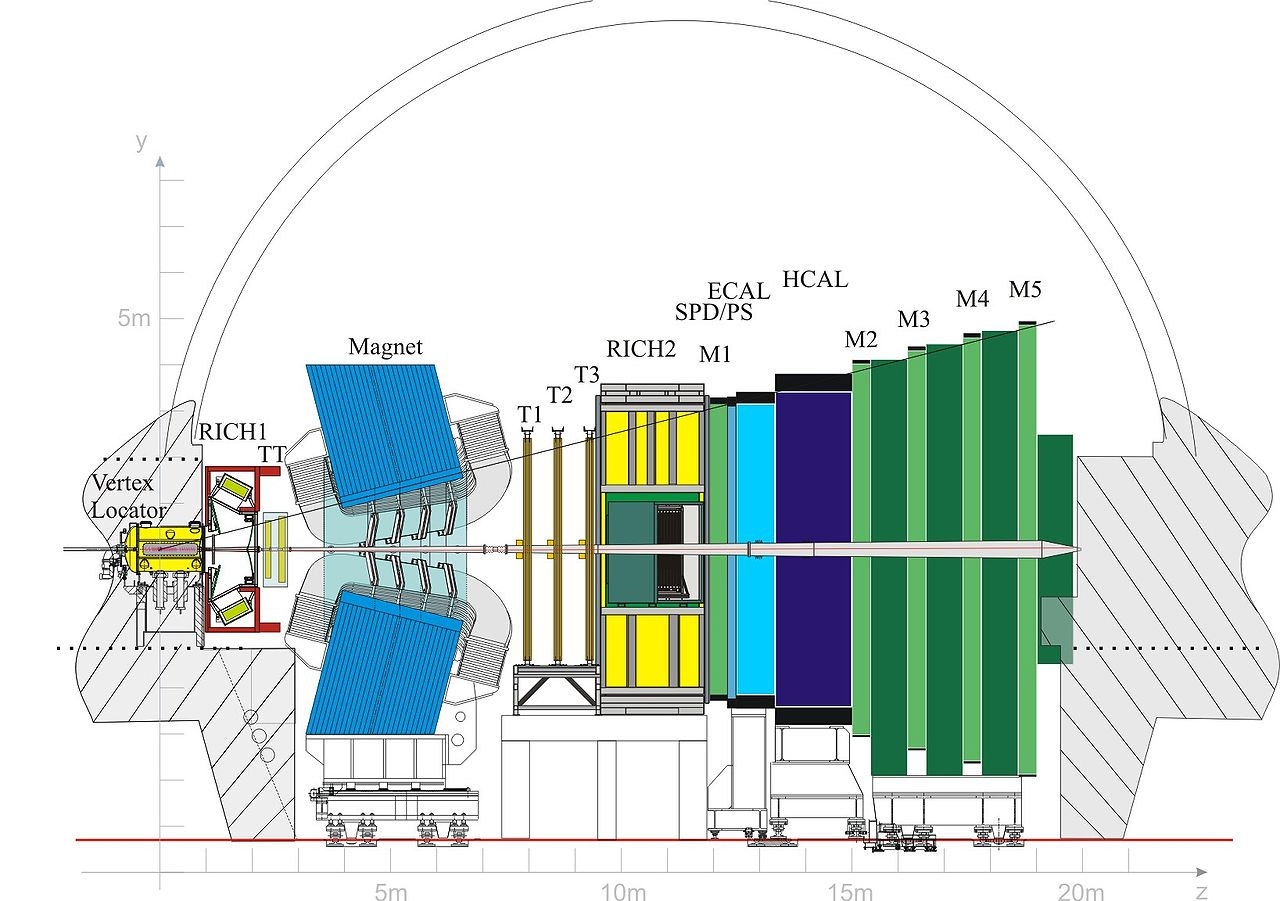
\includegraphics[scale=0.5]{LHCb_Det.jpg}
      \caption{The LHCb Detector along the bending plane.}
      \label{fig:LHCb_Collab}
    \end{figure}\FloatBarrier

    As B mesons are light (in comparision to other particles studied in the LHC), the decays products are produced at a shallow angle relivite the the beam pipe;
    this is the driving factor in the design of the exeperiment. 
    LHCb is a single arm forward spectormeter.
    Surrounding the point of collision is the \underline{Ve}rtex \underline{Lo}cator (VELO), this high precision detector uses silicon strips to detect ionising particles as they propogate from a collition and provides the coordinates of the particle in terms of R\footnote{Radial distance from the beam pipe.} and $\phi$\footnote{Asumthal angle.}.
    By reconstructing the paths of partics back to the intersection point, it can be identified wether or not the particular decay practicles are a product of the primary vertex\footnote{The position at which the protons collided.}, or a secondary vertex\footnote{The decay point of a short lived particle. i.e. B Meson.}.
    \par
    The Rich dectector, comprised of two subdectectors eitherside of the magnet, uses cherincov radiation to deduce the velocity of the particle. The silicon trackers, labeled TT and T1-3 in Figure~\ref{fig:LHCb_Collab}, calculate the angle deflection by the magnet. Be combining the velocity and angle of deflection, the mass, momentum and energy of the particles can be decuced from simple relitivistic kinematics.
    \par
    The meuon detectors, labeled M1-5 in Figure~\ref{fig:LHCb_Collab}, are important to detect muon's the detector. 
    This is of particular importance on LHCb as muons can be easily missidentified as charged pions, due to there simular mass.
    \par
    HCAl and ECAL, shown in Figure~\ref{fig:LHCb_Collab}, are hadronic and electric calorimeters respectively. 
    Both measure the total energy of incomming particles.
    As the calorimeters are absorbing of the particles they detect, any leptonic particle reaching the M2-5 muon detectors can be assumed to be a muon.
    Electrons and Photons are absorbed by the ECAl and any Tauons would have decayed long before reaching the far muon detectors.

      \subsection{LHCb Upgrade} % (fold)
      \label{sub:lhcb_upgrade}

      % subsection lhcb_upgrade (end)

      \subsubsection{VELO Upgrade}



      \subsubsection{The Role of FPGA's in the VELO Upgrade}

      


	\section{Scrambler}
\label{sec:scrambling_algorithms}

	Due to radiation levels inside the detector chamber, the main data processing takes place in a concrete bunker away from the detector.
	To facilitate this, 20 optical links (per module) are used to transfer the data from the front end VELO to the DAQ FPGA.
	When communicating data digitaly, the transferring module (TX) and the recieving module (RX) must have synchronised clocks.
	In this case, the GWT serialiser is the TX, and the DAQ is the RX.
	When achieving a synchronised clock, there are two main approaches:

	\begin{easylist}
		\ListProperties(Numbers=R,Margin=0.5cm,Align=fixed,FinalSpace=2em)
		% & Syncinize both the TX and RX from a single central clock - used in I$^2$C communication.
		& Transmit the TX clock with the data to the RX module - used in I$^2$C and SPI communication.
		& Use bit-changes in the data to continuously synchronise the RX clock.
	\end{easylist}

	The former of these options, although widely used in conventional electronics, requires a finely tuned clock accounting for all possible delays.
	The latter, while negating cons of the former, requires data with a high density of transitions to reduce the likelihood of a desynchronisation event.
	Because delays in the data are possible, the latter option has been selected.

	As mentioned, it is necessary to ensure that the data has a large density of transitions before being transmitted from the front-end detector to the DAQ module.
	However, as the majority of super pixel hitmaps are empty, the data has a bias towards \textit{`0'}s.
	This reduces the frequency of transitions in the data - increasing the probability of a desynchronisation event.
	It is therefore necessary to scramble the data prior to transmition and descramble the data in the LLI of the DAQ FPGA.
	\par
	Scrambling and later descrambling the data is not a trivial exercise.
	The scrambleing (TX) module and descrambling (RX) module must use a sychronised \textit{`key'}, that is used in both the scrambling and descrambling processes.
	In the FPGA, the \textit{`key'} is derived from the previous states of the data.
	There are two methods investigated for generating this \textit{`key'}:

	\begin{description}
		\item[Additive] The \textit{`key'} is generated by evolving the previous \textit{`key'} at each iteration of data using the incoming frame.
		\item[Multiplicative] The  \textit{`key'} is generated from the previous $n$ frames. (Here $n$ is a variable specific to the algorithm).
	\end{description}

	\subsection{Scrambler Options}
	\label{sub:scrambler_options}

		Three scrambling algorithms have been considered:

		\begin{description}
			\item[Additive Scrambler] \hfill \\
				This scrambler was originally implemented and used two sets of two-input XOR logic gates.
				As the name implies, this scrambler used additive key generation which is dependent on all previous input frames since the last reset signal.

			\item[Intermediate Scrambler] \hfill \\
				Created by Karol Hennessy, and deriving its name arbitrarily from the order of consideration, this multiplicative scramber combines the current and previous frames to generate the \textit{`key'}.
				Therefore, in the event of desynchronisation, only two frames are lost before the \textit{`key'} is automatically recovered.
				This feature alone is a significant improvement over the Additive Scrambler.

			\item[VeloPix Scrambler] \hfill \\
				This is the current implemented scrambling algorithm in the DAQ and VeloPix code.
				Like the Intermediate Scrambler, it uses multiplicative \textit{`key'} generation.
				However, the VeloPix scrambler is compatible with further constraints enforced by the ASIC, including the number of combinational logic operations.
				The Intermediate Scrambler was design purely for simulation purposes and as such does not meet the additional ASIC constraints.
		\end{description}


	\subsection{Cross Checks} % (fold)
	\label{sub:cross_checks}
		The main priority when scrambling data, is ensuring that the data is recoverable.
		For all three scramblers, the algorithm was synthesised in Quartus \cite{ref:quartus} and simulated in Modelsim \cite{ref:modelsim}.
		The aim of synthesising and simulating the scramblers in these programs was to ensure that the design was both physical in terms of on-board logic gates, and to check that the scrambled data was recoverable, respectively.
		\par
		Furthermore, a C++ simulation was created for the three scramblers.
		This simulation had two main purposes;
		firstly to cross check the output of the C++ against the Modelsim simulations;
		secondly to simulate the scrambler over a much larger sample of data as Modelsim simulations are less time effecient.
		In addition to the cross checks, the C++ code allowed for the injection of a desychrnonisation event, in which the \textit{`key'} is lost.
		As expected, the Additive Scrambler was unable to recover any data post desychrnonisation, however the intermediate and VeloPix scarmblers both recovered the \textit{`key'} after two frames and continued to decode data.

	% subsection cross_checks (end)

	\subsection{Algorithm Analysis}
	\label{sub:algorithm_analysis}

		For analytical purposes, it is assumed that fully scrambled data is indistinguishable from randomly generated data. 
		For this reason, the three algorithms are not only tested against each other and pre-scrambled simulated QWT data but also randomly generated binary.
		The randomly generated data was created using the Python \textit{`random'} library, selecting a \textit{`0'} or \textit{`1'} with equal probability.
		While the Python \textit{`random'} library is only pseudo-random, on the scale of this application (i.e. $>>$ 100,000 frames), it is sufficient for these purposes.
		\par
		A more mathematically rigorous approach, however, is to evaluate the system abstractly in the framework of statistical physics.
		In this abstraction, the 120 bit frame (with the header and parity removed)  is considered an ensemble; 
		microstates are the particular form of the frames;
		and macroscopic quantities can be calculated by averaging a large number of frames.
		For the analysis outlined in section \ref{subsub:messurements_of_the_algorithms}, predictions will be made using these principles and outlined in section \ref{subsub:statistical_predictions}.
		\par
		In the context of the statisical model, it is reasonable to consider the degree of \textit{`scrambled-ness'} analogous to entropy.	
		This analogy is not disimilar to the common interpretation of entropy as a measure of disorder. 
		From Boltzman's equation for entropy,

		\begin{equation}
			S \propto ln(\Omega)
			\label{eqn:boltzman}
		\end{equation}

		where $\Omega$ is the number of microstates assosiated with the macrostate, we learn that this state of maximum entropy is a macrostate with the maximum number of assosiated microstates.
		\par
		The entropic argument of Equation~\ref{eqn:boltzman} is not only mathematically founded. 
		For a scramble algorithm to hold for all possible data sets, it must also be capable of outputting all possible permutations. 
		As such, assuming all possible outputs are equally likely, the count of each macroscopic output will be proportional to the number of microstates associated.

		\subsubsection{Measurements of the Algorithms} 
		\label{subsub:messurements_of_the_algorithms}

			To compare the efficiency of the three algorithms in section \ref{sub:scrambler_options}, the algorithms where run over the same input data and compared for the following measures:

			\begin{description}
				\item[Number of Transitions Per Frame] \hfill \\
					This measure counts the total number of bit transitions (i.e. $bit(n) \neq bit(n-1)$) in a 120 bit frame. 
					The header and parity information was not included as they are not scrambled.
					This is an important test as one of the roles of the scrambler is to maximise the number of transitions.

				\item[Common Bit Chain Length] \hfill \\
					One of the downfalls of the `Number of Transitions Per Frame' analysis is that the two hypethetical 20 bit frames,

					\begin{enumerate}[a)]
						\item \textsc{10101010101111111111},
						\item \textsc{10011001100110011001},
					\end{enumerate}

					both with 10 transitions, are considered to be equal. However, (b) is clearly a more suitable output for data transfer as (a) has a large probability of desynchronisation due to the long chains of \textit{`1'}s in the rightmost bits.
					It is therefore also necessary to evaluate the length of common bit chains within the scrambled data as shorter chains are more suitable for data transfer.

				\item[Bit Asymmetry] \hfill \\
					Pre-scramble, the data had a large bais towards \textit{`0'}s due to the majority of the hitmaps being empty.
					Scrambled data, via entropic arguments, \textit{should} show zero bias eitherway.
					Therefore, by investigating how the number of \textit{`1'}s - \textit{`0'}s evolves over many frames, any bias in the scrambler can be found.

			\end{description}	

		\subsubsection{Statistical Predictions} % (fold)
		\label{subsub:statistical_predictions}

			\begin{description}
				\item[Number of Transitions Per Frame] \hfill \\
					
					Consider a particle in a symmetric, discrete time-dependent, two state system,

					\begin{equation}
						p_0(t) = p_1(t) = 0.5 \quad : \quad \forall\ t \in \mathbb{N},
					\end{equation}

					At each time iteration,

					\begin{equation}
						p_{i \to j}(t) = 0.5 \quad : \quad i,j = [0\ 1], \quad \forall\ t \in \mathbb{N}.
					\end{equation}

					However, assuming zero bias and detailed balance, as $p_{1 \to 0}(t)$ is equal in both probability and importance to $p_{0 \to 1}(t)$, the probability of a bit change shall henceforth be refered to as $p_{\tau}(t)$.
					\par
					Over an $n$ step process, analogous to an $n$ bit frame, the probalility distribution of the number of transitions $N_\tau$ is given by Binomial statistics,

					\begin{equation}
						f(N_{\tau}) = \frac{n!}{N_{\tau}!(n-N_{\tau})!}\ p^{N_{\tau}}\ (1 - p)^{n-N_{\tau}}
					\end{equation}

					Simplified for the special case $p = p_{\tau} = 0.5$,

					\begin{equation}
						f_{\tau}(N_{\tau}) = \frac{n!}{N_{\tau}!(n-N_{\tau})!}\ (p_{\tau})^{n}
						\label{eqn:transition_propability_dencity}
					\end{equation}

					For $n = 120$, we can calculate,

					\begin{equation}
						<N_\tau>^{Binomial} \ = \sum_{N_{\tau}=0}^{n-1} N_{\tau}\ f(N_{\tau}) = n\ p_{\tau} = 60
						\label{eqn:tansition_expectation}
					\end{equation}

					\begin{equation}
						\sigma_{N_\tau}^{Binomial} = \sqrt{ n\ p_{\tau}^2} = 5.48
					\end{equation}

					Furthermore, when considering the entropic argument of equation \ref{eqn:boltzman}, the number of microstates corresponding to each macrostate $N_\tau$ can be related to equation \ref{eqn:transition_propability_dencity},

					\begin{equation}
						\Omega_\tau \sim \frac{n!}{N_{\tau}!(n-N_{\tau})!}
					\end{equation}

					\begin{equation}
						<N_\tau>^{Entropic} = MAX[S_\tau] = MAX[\Omega_\tau]
					\end{equation}

					This can be numerically solved,

					\begin{equation}
						<N_\tau>^{Entropic}\ = 60
						\label{eqn:n_t_entropic}
					\end{equation}

					While the result of equation \ref{eqn:n_t_entropic} does not contibute anything new, it is important as a \textit{`sanity check'}.
					Because the system can be described as in section \ref{sub:algorithm_analysis}, it would indicate a problem in the theoretical framework if the result did not match.


				\item[Common Bit Chain Length] \hfill \\
					
					The probability of a chain of length $n$ is,

					\begin{equation}
						p_n = p_1(1 - p_\tau)^{n-1}, \quad : \quad n \in \mathbb{N}, \quad n > 1
					\end{equation}

					where $p_1$ is the number of chains of length 1. 
					As $p_1 = N_0 (1 -p_\tau)$, where $N_0$ is the total number of chains,

					\begin{equation}
						\frac{N_n}{N_0} = (1 - p_\tau)^n, \quad : \quad n \in \mathbb{N}, \quad n > 1
					\end{equation}

					where $N_n$ is the number of chains of length $n$.
					Taking the logarithm of both sides,

					\begin{align}
						log\left(\frac{N_n}{N_0}\right) &= n\ log(1 - p_\tau), \nonumber \\
 						log(N_n) &= n\  log(1 - p_\tau) + log(N_0).
 					\end{align}

					Therefore, for a graph of $log(N_n)$ against $n$ for a large sample of data, the gradient would be $log(1 - p_\tau)$.
					In this case, as $p_\tau = 0.5$, 

					\begin{equation}
						log(1 - p_\tau) = -0.30\ .
						\label{eqn:log_chain_length_gradient}			
					\end{equation}

				\item[Bit Asymmetry] \hfill \\
					
					$A_{1,0}$, the asymmetry of \textit{`1'}s and \textit{`0'}s is defined as,

					\begin{equation}
						A_{1,0} = N_1 - N_0,
						\label{eqn:a_def}
					\end{equation}

					where $N_1$ and $N_0$ are the number of \textit{`1'}s and \textit{`0'}s respectively.
					We can consider the evolution of $A_{1,0}$ with frame $t$ of size $n$ as a stochastic iterative map with zero deterministic growth \cite{ref:stockastic_physics},

					\begin{equation}
						A_{1,0}(nt + n\ \Delta t) = A_{1,0}(nt) + \mathcal{N}(nt).
					\end{equation}

					Where $\mathcal{N}$ is an independant random variable picked from a gaussian distribution. While $A_{1,0}(t) \in \mathbb{Z}$, in the limit of large $nt$ we can approximate that $A_{1,0}$ is continous. 
					\par
					If we consider the moments of $A_{1,0}$,

					\begin{align}
						\label{eqn:A_moment1}
						<A_{1,0}(nt = M\ n\ \Delta t)> & = \sum_{m = 0}^{M -1}  \mathcal{N}(m\ n\ \Delta t), \\
						\label{eqn:A_moment2}
						<A_{1,0}(nt = M\ n\ \Delta t)^2> & = \sum_{m=0}^{M-1} \sum_{m'=0}^{M-1}  \mathcal{N}(m\ n\ \Delta t) \mathcal{N}(m'\ n\ \Delta t)\ \delta_{mm'} \nonumber \\
						&= \sum_{m=0}^{M-1} < \mathcal{N}(m\ n\ \Delta t)^2 >.
					\end{align}

					Clearly, in Equation \ref{eqn:A_moment1}, $<A_{1,0}> = 0$. In Equation \ref{eqn:A_moment2}, we assume the variance is of form $(n\ \Delta t)^\alpha$ \cite{ref:stockastic_physics}. Then,

					\begin{equation}
						<A_{1,0}(nt = M\ n\ \Delta t)^2>\ = M (n\ \Delta t)^\alpha.
						\label{eqn:A_moment3}
					\end{equation}

					Running the analysis over the frames $t = 0$ to $t_f$, the number of bits sampled is $M = {t_f / n\ \Delta t}$. Substituting this into Equation \ref{eqn:A_moment3},

					\begin{equation}
						<A_{1,0}(nt = M\ n\ \Delta t)^2>\ = t_f\ (n\ \Delta t)^{\alpha -1}.
					\end{equation}

					Considering the three cases of $\alpha$ in the approximation of continous $n \Delta t$:
					
					\vspace{1em}

					\begin{easylist}[itemize]
						% \ListProperties{Margin=2cm,Align=fixed,FinalSpace=2em}
						& $\bm{\alpha > 1}$: Here $A_{1,0} \to 0$ as $\Delta t \to 0$.
						& $\bm{\alpha < 1}$: Here $A_{1,0} \to \infty$ as $\Delta t \to 0$.
						& $\bm{\alpha = 1}$: This is the only sensible choice.
					\end{easylist}
					
					\vspace{1em}

					With $\alpha =1$,

					\begin{equation}
						<A_{1,0}(nt = M\ n\ \Delta t)^2> = M (n\ \Delta t).
					\end{equation}

					And thus,

					\begin{equation}
						\sigma_{A_{1,0}} = \sqrt{<A_{1,0}^2> - <A_{1,0}>^2} = \sqrt{<A_{1,0}^2>} = \sqrt{n\ \Delta t}.
					\end{equation}

			\end{description}	

		\subsubsection{Results of Analysis}
		\label{subsub:algorithm_results}
			\begin{SCfigure}%[ht]
				\centering
				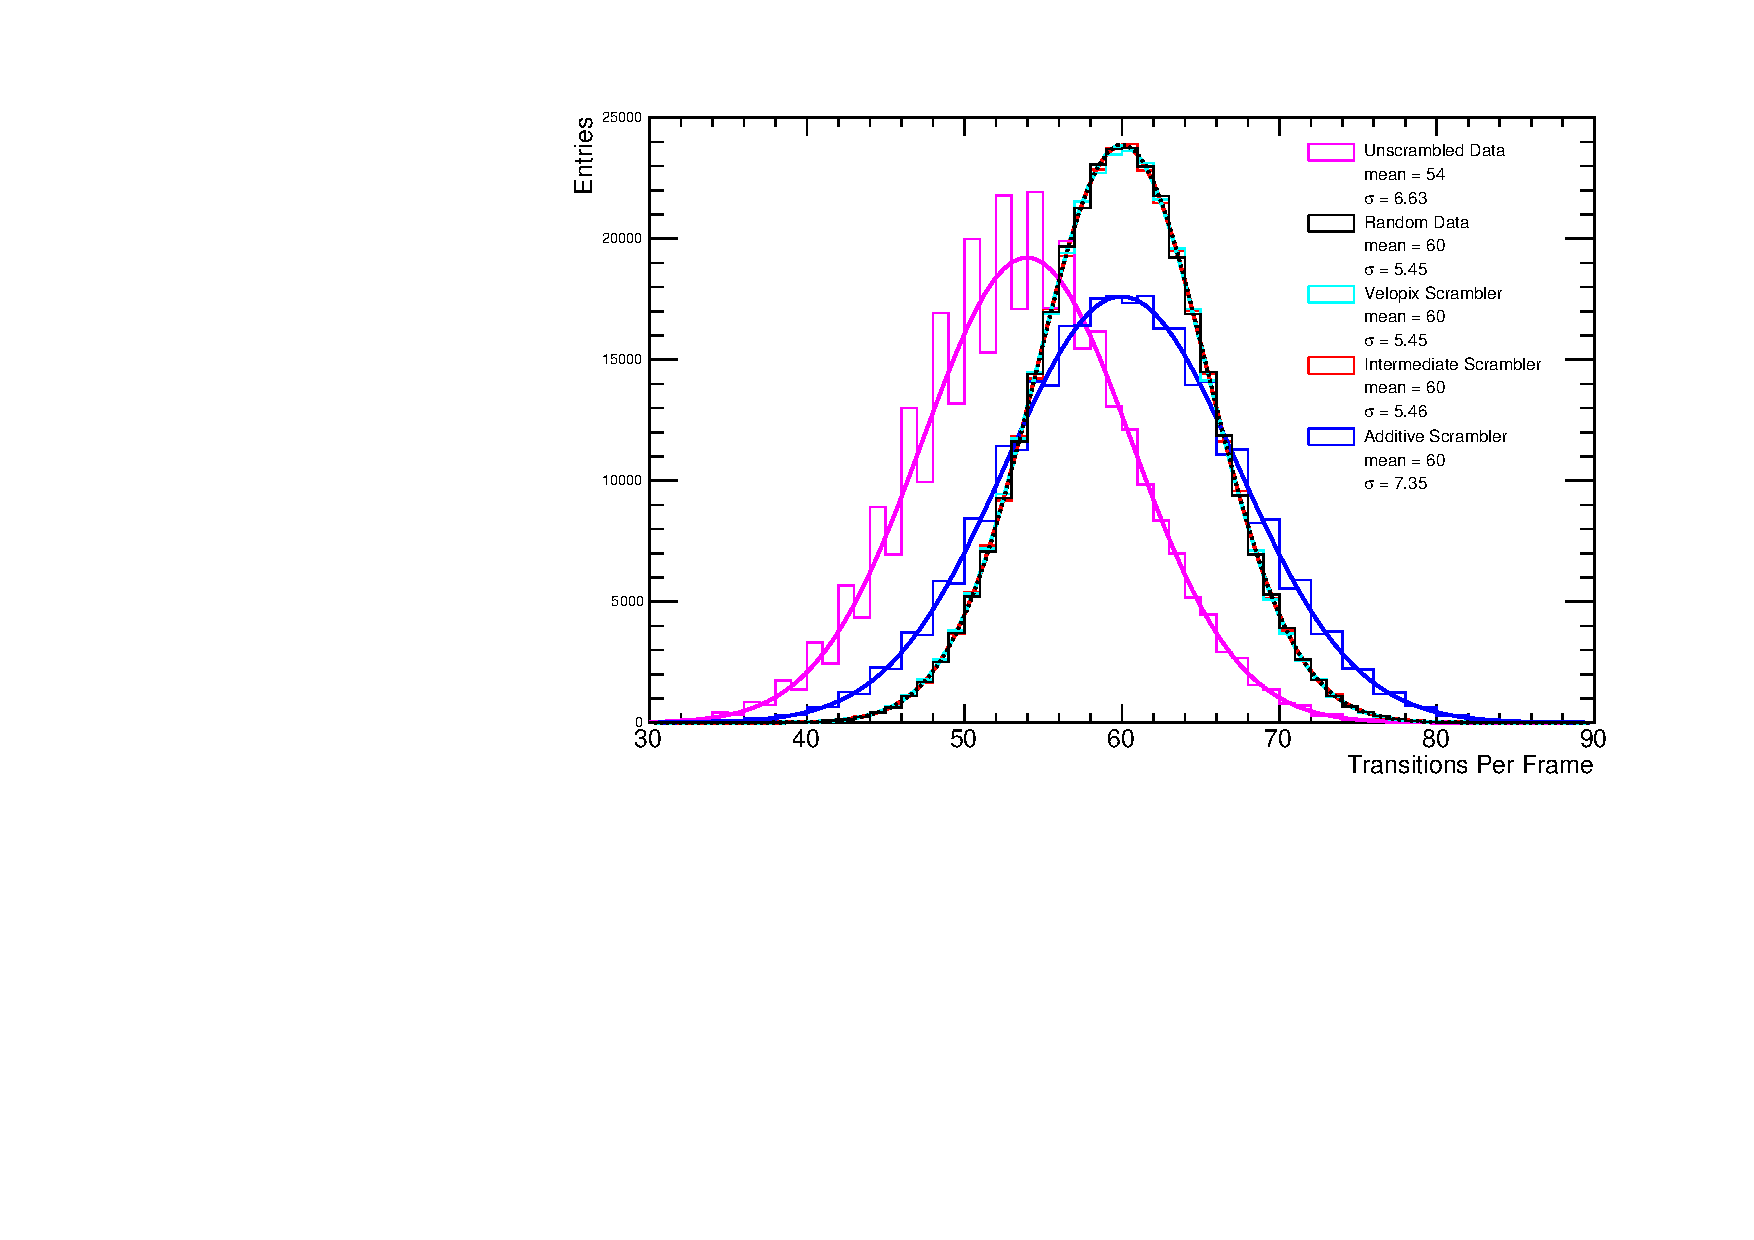
\includegraphics[width=0.7\textwidth]{Transition_Histogram_update}
				\caption{Results of the \textit{`Number of Transitions Per Frame'} analysis. The results for the Random Data, Intermediate Scrambler and VeloPix Scrambler overlap.}
				\label{fig:transitions_per_frame}
			\end{SCfigure}
			\par
			\begin{SCfigure}%[ht]
				\centering
				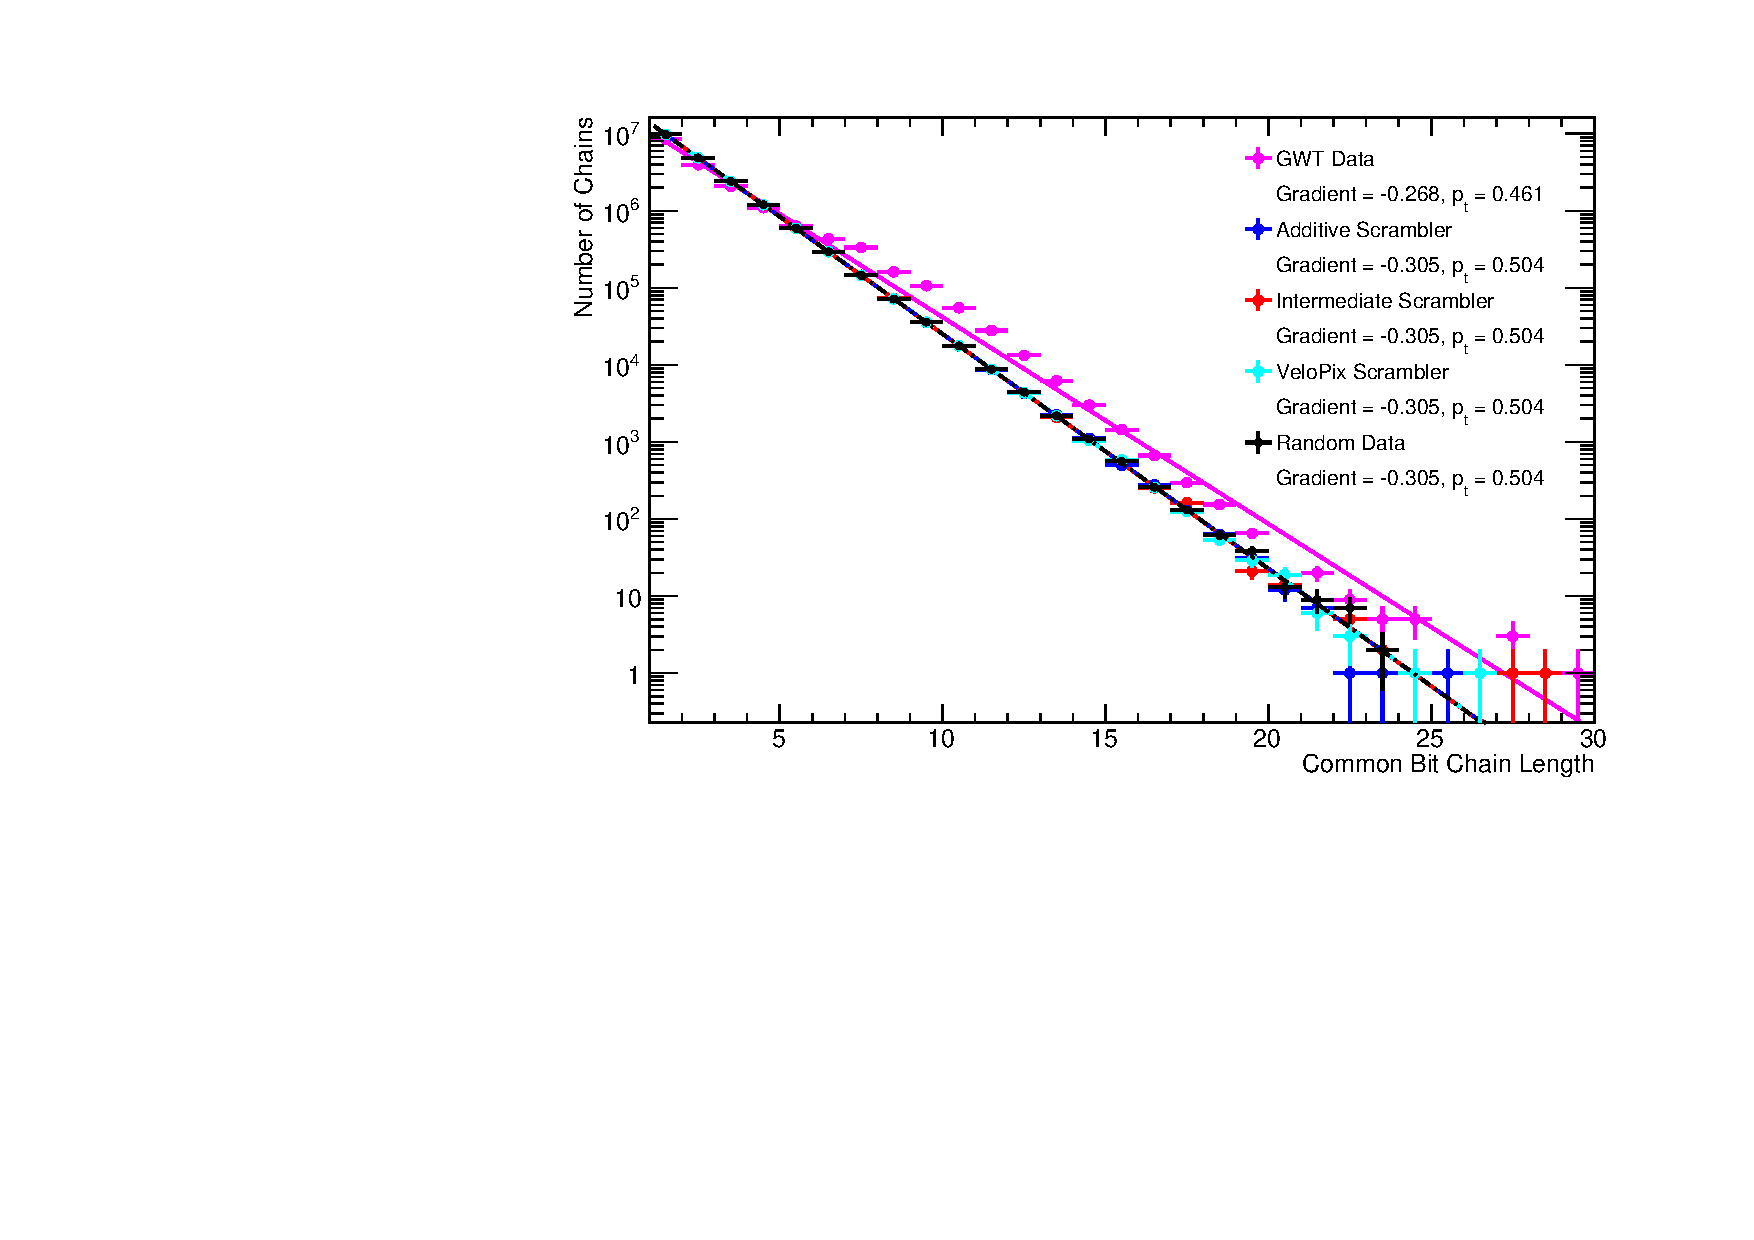
\includegraphics[width=0.7\textwidth]{Chain_length}
				\caption{Results of the \textit{`Common Bit Chain Length'} analysis. The results for the Random Data, Additive Scrambler, Intermediate Scrambler and VeloPix Scrambler overlap.}
				\label{fig:chain_length}
			\end{SCfigure}
			\par
			\begin{figure}[ht]
				\centering
				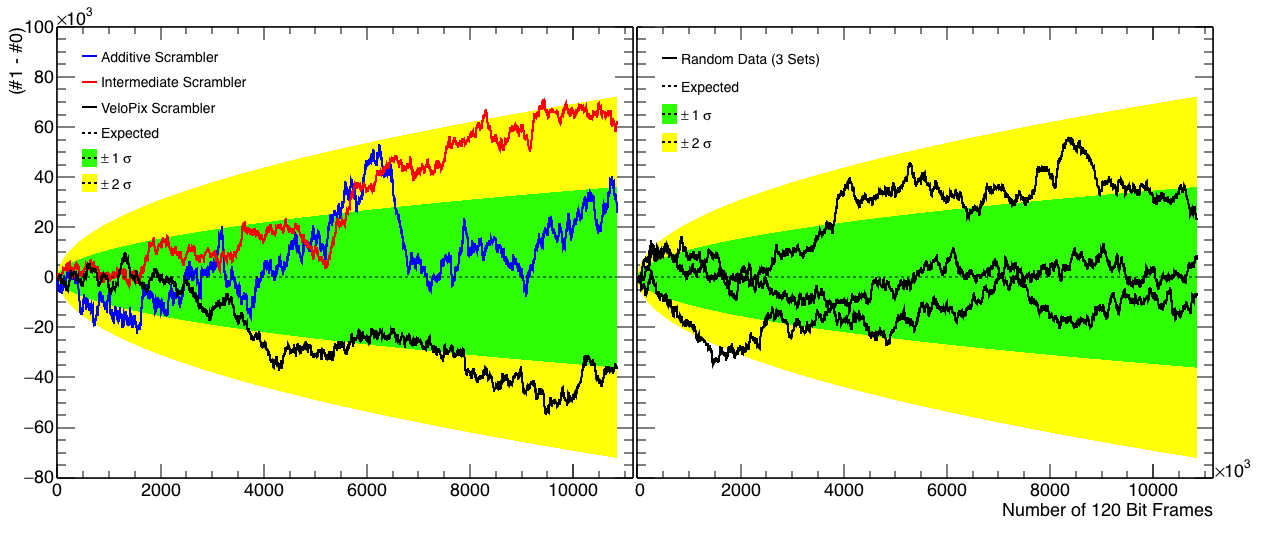
\includegraphics[width=1\textwidth]{Balance_graph_cropped}
				\caption{The results of the \textit{`Bit Asymetry'} analysis.}
				\label{fig:bit_asym}
			\end{figure}

			The results from the \textit{`Number of Transitions Per Frame'} analysis, shown in Figure~\ref{fig:transitions_per_frame}, show a strong similarity between the Intermediate and VeloPix Scramblers with the randomly generated data. 
			These results are within 1\% agreement with the theoretical predictions for $<N_\tau> = 60$ and $\sigma_{N_\tau} = 5.48$, made in Section~\ref{subsub:statistical_predictions}. 
			The remarkable consistancy between the theoretical predictions and the randomly generated data provides confidence in both the theory, and the scrambled nature of the Intermediate and VeloPix scrambler outputs.
			\par
			For the \textit{`Common Bit Chain Length'} analysis all three scramblers; the random data, and the theoretical predictions are consistant to within 1\%. 
			Comparing the results for the Additive Scrambler, it is shown that while the frequency of longer chains is consistent with random data, the variance of transitions is larger than predicted. 
			Thus, the long and short trains are more locally clustered. 
			\par
			The \textit{`Bit Asymmetry'} of each scrambler, shown in Figure~\ref{fig:bit_asym}, is consistent with the theoretical prediction. 
			The deviation of $A_{1,0}$ for the predicted mean of 0 is fully consistent with stochastic noise. 
			The random data also shows consistency. 
			This gives confidence in the assumptions made in Section~\ref{subsub:statistical_predictions}.		
 			% \par		
 			% One notible feature of Figure\ref{fig:bit_asym} is the steap grandient of the additive scrambler a $t \sim 6.10^6$.		
 			% However, as the data stays within the theoretical limits and the \textit{`drop'} is of approximatly $\Delta A_{1,0} \sim 60.10^3$ over the range $n\ \Delta t \sim 1.2.10^8$ it would be difficult to construnct any argument claiming that this feature is of statistically significance.

	\subsection{Conclusion}

		\begin{table}[h]		
 			\centering		
 			\begin{TAB}(r)[7pt]{l|cc:cc}{c|c:ccc:cc}		
 							           & $<N_\tau>$ & $\sigma_{N_\tau}$ & Gradient  	& $p_\tau$    \\		
 				GQT data  		       & 54      	& 6.63           	& -0.268 		& 0.460 \\		
 				Additive Scrambler     & 60      	& 7.35           	& -0.305 		& 0.504 \\		
 				Intermediate Scrambler & 60      	& 5.45           	& -0.305 		& 0.504 \\		
 				Velopix Scrambler      & 60      	& 5.46           	& -0.305 		& 0.504 \\		
 				Random Data            & 60      	& 5.45           	& -0.305 		& 0.504 \\		
 				Theoretical Prediction & 60      	& 5.48           	& -0.3 			& 0.5   			
 			\end{TAB}		
 			\caption{The combined results of the algorithum analysis.}		
 			\label{tab:comb_results}		
 		\end{table}		
 		
 		The consistency of random data and the theoretical predictions justifies the assumptions and approximations made in Section~\ref{sub:algorithm_analysis} and Section~\ref{subsub:statistical_predictions}. 
 		Furthermore, the confirmation of the statistical model allows for accurate comparisons to be made from predicted values and their measured counterparts.		
 		\par		
 		The Additive Scrambler, while consistent with the \textit{`Chain Length'} and \textit{`Bit Asymmetry'} analysis, has a variance in the transition frequency that leads to the conclusion that long and short chains are locally clustered. 		
 		This is not ideal for data transfer. 		
 		Many sequential long chains increase the probability of TX-RX clock desynchronisation. 		
 		Furthermore, the additive scrambler will not recover from this loss of synchronisation, as the \textit{`key'} will never be recovered without a common reset signal.		
 		\par		
 		The Intermediate Scrambler produced an output consistent with random data. 		
 		This makes the algorithm suitable for data transfer.		
 		As already mentioned, however, the scrambler is designed for computer simulation.		
 		As such, it is not suitable for implementation as it does not meet the addition requirements of the ASIC.		
 		\par		
 		The VeloPix Scrambler, like the Intermediate Scrambler, produces a statistically scrambled output.		
 		Furthermore, the algorithm is inline with the additional requirments of the ASIC.		
 		As such, it is ideal for implementation, and hence is currently the choice algorithm for use in the 2019 VELO upgrade.









	\section{Event Isolation Flagging}
	
	One challenge of increasing the readout speed of the detector is processing the data that is produced.
	Because of this, any pre-computer data processing that is possible reduces the load and processing time of the computer system.
	One area where the DAQ's FPGA will be used for this purpose is in \underline{E}vent \underline{I}solation \underline{F}lagging (EIF).
	\par
	Particles traversing the VELO have a probability that they will pass though the boundary of two or more Super Pixels.
	This will cause multiple SPPs to be created for the same particle path.
	As such, the reconstruction of the particle's path is a more complicated process than a particle path that only interects with one SP.
	\par
	The aim of EIF is to identify the SPPs that completly describe the paticles interaction with the module and flag that event as isolated.
	These flagged events will allow the computer systems to prioritize these easier to reconstruct paths.
	This reduces event pile up the computer network.

	\subsection{Time Sorting Data}

		Frames arriving the DAQ from the GWT are not time ordered.
		When fully implimented, the LLI will have time sorted the data before the EIF.
		However, the provided simulated data of the VELO not time ordered.
		\par
		In order to test any EIF development, it is necessary to time order the simulation data.
		This was done using a python script that sorted the SPPs into lists according to BCID.
		The script has three main phases:

		\begin{easylist}
			& Read in a SPP and retrieve BCID.
			& Add the SPP to the correct list according to BCID.
			& Print the list of opposite BCID (i.e. input SPP's BCID + 124, accounting for BCID 256 rolling over to 0) to file.
			& Print the list of opposite BCID to file. (The opposite BCID is the BCID 124 away from the BCID read in, taking the result modulo 256.)
		\end{easylist}

		As not all BCID's were present, measures were put in place to ensure all BCID lists were outputed in time order, preventing lists containing SPPs from two or more bunch crosses. The time order of the data was tested and confirmed as correct.
		% \par
		% One advantage of this process is that, regardless of the number of isolated events, the data no longer needs to be sorted by the computer network.
		% This further reduced the computational load on the computers.

		\subsection{Bubble Sorting}

		Bubble sorting is the process of sequentially comparing adjacent elements of a list and swapping the element if necessary.
		For example, if sorting into acsending order and comparing the value 5 and 3, a swap would be needed.
		However, comparing 3 and 5 in the same example would not need a swap.
		When sorting an arbitrary list, we can define an `even-odd' comparison as one comparing an even placed element with an odd one (i.e. element 4 with element 5).
		An `odd-even' comparison is the logic opposite (i.e. element 5 with element 6).
		\par
		The first step in EIF is to sort all the SPP's that correspond to the same bunch crossing (Henceforth referred to as a \textit{`data train'}) by their row in the ASIC.
		\par
		Bubble sorting, when implemented in series processing, is a relatively slow sorting algorithm.
		At worst case, Bubble sorting requires $n^2$ iterations to complete the sort of a list of size $n$.
		However, FPGAs can easily parallel proccess.
		By making $\frac{n}{2}$ comparisons simultaniously (all even-odd or odd-even pairs), FPGA Bubble Sorting in the worst case scenario only requires $n$ iterations. This is made clear in Figure~\ref{fig:sorting}.

		\begin{figure}[ht]
			\centering
			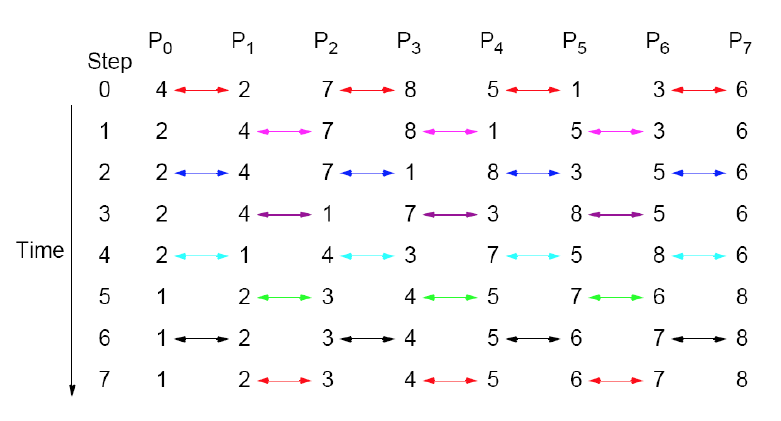
\includegraphics[width=0.7\textwidth]{sorting_diagram}
			\caption{A diagram showing Bubble Sorting in an FPGA.}
			\label{fig:sorting}
		\end{figure}

	\subsection{Isolation Checking}

		Once the data train is sorted by row, each SPP in the train can be compared against its adjacent SPP's.
		If the SPP is separated by more than 1 row to both adjacent SPP's, the event is isolated.
		The SPP is then stored as a 31 bit SPP, with the new bit added as the least significant bit (shifting the original SPP 1 bit in significance), with the new bit signalling 1 for isolated and 0 for non-isolated. 

	\subsection{Data Train Overflow} % (fold)
	\label{sub:data_train_overflow}
		
		One limitation of EIF in an FPGA is the limitation on resources. 
		The logic systems are static in design and, as such, there is a natural need for a cap on the size of the data train that the EIF system can accept - specifically for the bubble sorting.
		Because of this limitation, the EIF system is required to implement an overflow system that will reject data trains above a pre-determined limit, and move them to the next step of the LLI without proccessing them.
		This system is also required to bypass data if a data train arrives at the EIF system before the previous train has been processed - preventing pile-up.
		\par
		In order to investigate the limit needed for the overflow, the distribution of data train sizes was investigated. For each ASIC, a graph similar to those in Figure~\ref{fig:asic_datatrain} can be created.

		\begin{figure}[h]
			\centering
			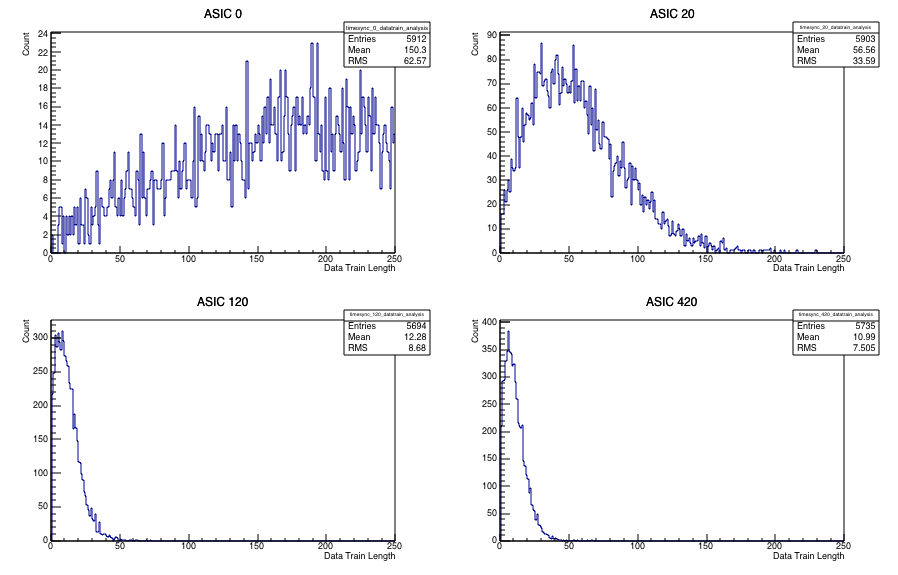
\includegraphics[width=\textwidth]{asic_datatrain_length}
			\caption{The data train length distribution of 4 ASIC chips.}
			\label{fig:asic_datatrain}
		\end{figure}
		\par
		\begin{figure}[h]
			\centering
			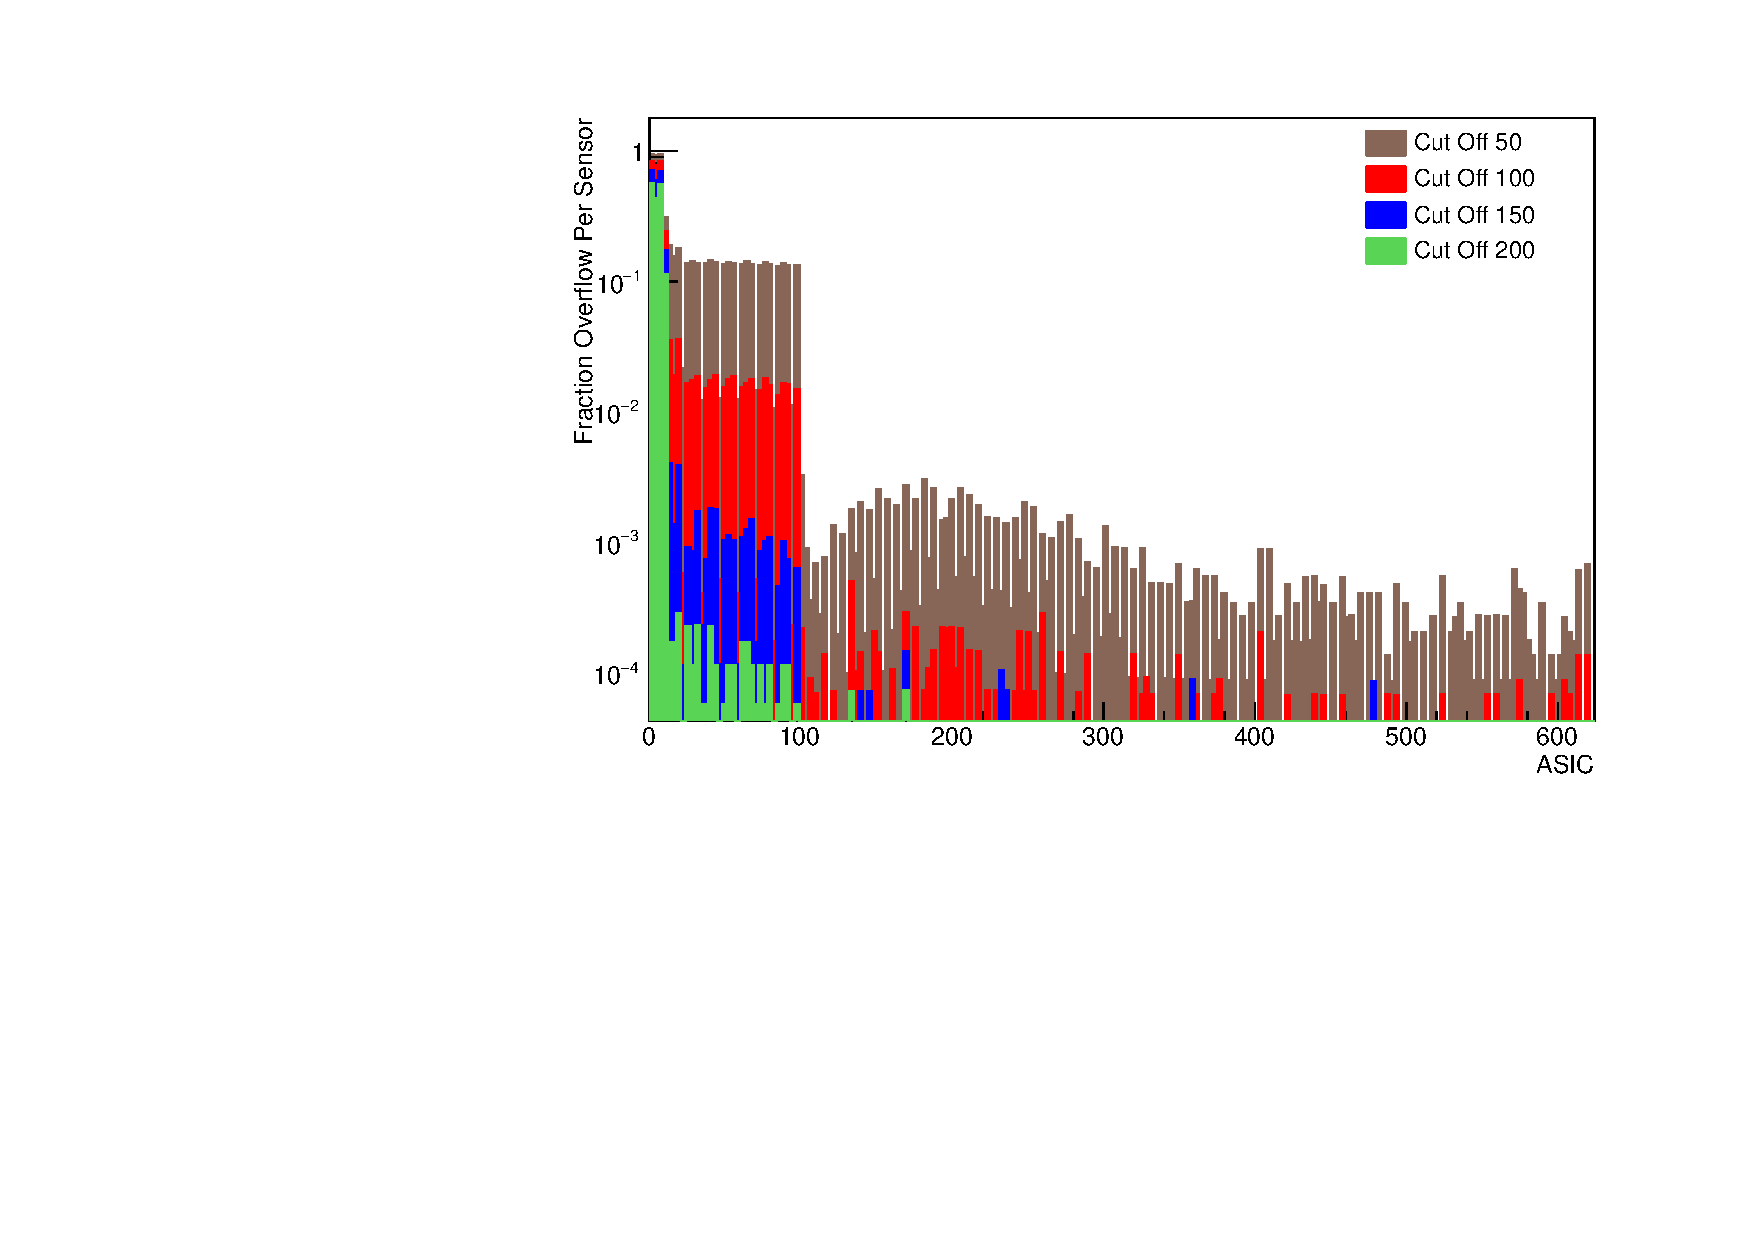
\includegraphics[width=0.7\textwidth]{overflow_graph.pdf}
			\caption{fraction of overflow data trains for four overflow limits.}
			\label{fig:overflow_franction}
		\end{figure}\FloatBarrier
		More important, however, is the fraction of data trains over the bypass limit.
		For four hypothetical limits, the fraction of overflow data trains was calculated from the VELO simulated data, and is shown in Figure~\ref{fig:overflow_franction}.
		This analysis, however, raises questions beyond that of the overflow limit.
		The ASICs below 100 show no simulatity to those above 100.

		\begin{figure}[h]
			\centering
			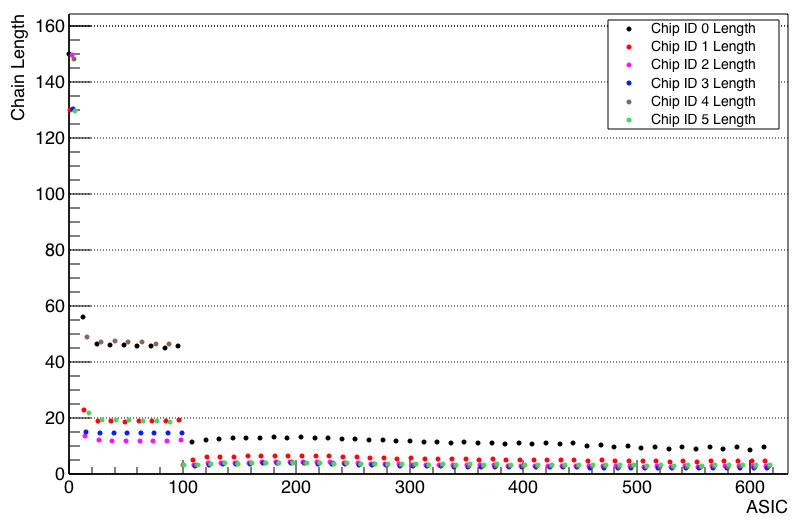
\includegraphics[width=0.49\textwidth]{Mean_ASIC_Graph_Chip}
			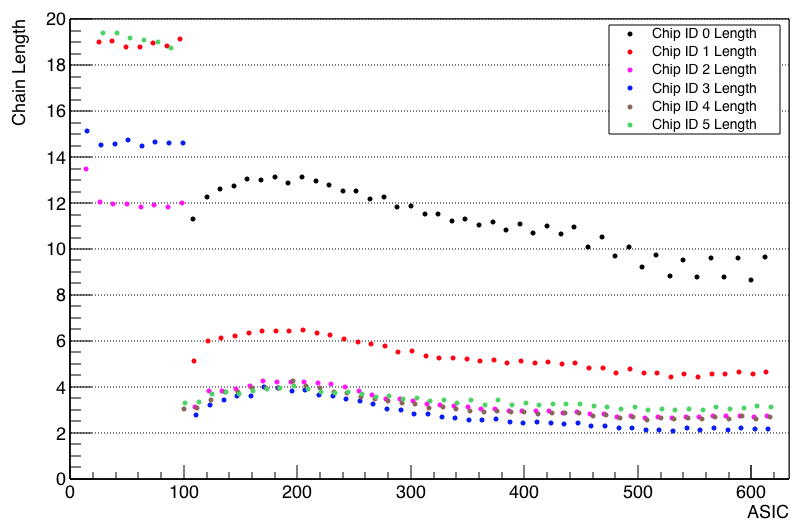
\includegraphics[width=0.49\textwidth]{Mean_ASIC_Graph_Chip_lower_values}
			\caption{The mean data train length for each ASIC, coloured by the chip number.}
			\label{fig:asic_structure}
		\end{figure}\FloatBarrier
		Further investigations as to the structure of the simulated data is shown in Figure~\ref{fig:asic_structure}.
		Here the data is partitioned by the position of the ASIC chip in the module.
		From this we learn that large variance in the data (ASIC number $>$ 100) is due to the ASICs position on the module.
		This result is expected as the ASICs closer to the beam line will detect more particle paths.
		However, this structure is not consistaent across the ASIC's pre and post 100.
		It can be concuded that the simulated data contains a \textit{`bug'}.
		This \textit{`bug'} is now being reviewed by the creators of the simulation. 
		No further analysis can be continued on setting an overflow limit until this \textit{`bug'} has been properly investigated.

		% subsection data_train_overflowa (end)

	\subsection{Current Stage of Development} 
		The EIF system is still currently in active VHDL development.
		The current developmental code is still in a stand alone format and not intergrated with the master LLI code.
		Currently created and ready for stand alone testing, is a bubble sorting module with data in and out systems.
		The module consists of a top level control entity and a comparison/swap sorting entity.
		The control entity forms a feedback loop passing the ouput of the sorting enity back into its input at each step.
		At each step, the parity of comparison is changed (i.e. odd-even to even-odd).
		\begin{figure}[h]
			\centering
			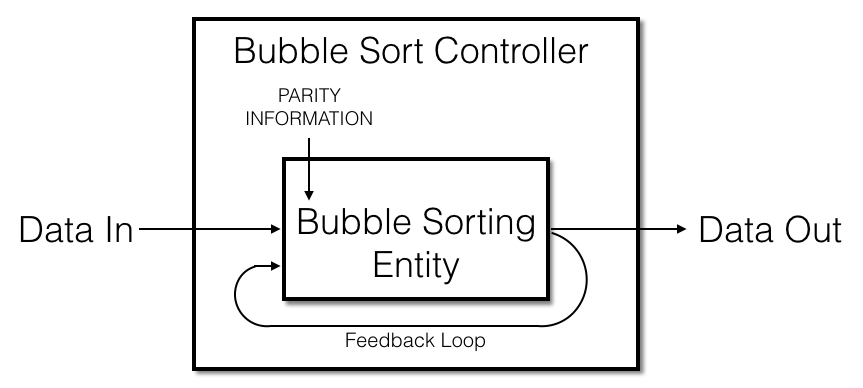
\includegraphics[width=0.65\textwidth]{bubblesort_modual}
			\caption{Data from for the developmental bubble sorting module.}
			\label{fig:bubble_data_flow}
		\end{figure} \FloatBarrier
		\par
		This process continues until the input and output of the sorting module is identical for two subsequent steps.
		At this point the data is sorted and passed to the output.
		The data flow is more simply demonstrated in Figure~\ref{fig:bubble_data_flow}.
		\par
		Once testing of the bubble sorting is complete and the simulated data bug is fixed, the EIF will be expanded to include Isolation Flagging and an overflow, as discussed.
		Once the stand alone system is complete, it will be intergrated into the LLI master code and modified to comply with the LLI data management systems.
		\FloatBarrier

	\section{Future Development}

	Once the current areas of FPGA development discussed in this document are complete, focus can be directed on areas of the LLI still in active developemt.
	One such area is in the processing of incoming data from the optical links into frames in the DAQ, currently being worked on by a colleague in Manchester University.
	However, due to the nature of the development being spead over many European countries, reliably predicting the next step in development is a not possible.
	\par
	Once the FPGA development is complete and the VELO upgrade is implemented in 2019, the more accurate VELO data will allow for greater statistical analysis and more significant results.
	This is of particular interest for rare processes, such as CP violation, which are largely dominated by statistical error with the current LCHb data.



	%\section{Conclusion}

	This is the Conclusion

	% ----- Acknowledgements & Bibliography ----- %
	\section{Acknowledgments}
	I would like the acknowledge Pablo Rodriguez, Marco Gersabeck and Chris Parkes for their continued support and supervision.
	I also acknowledge Benjamin Jeffrey for his equal role in the Scrambler Analysis and Event Isolation Flagging.
	I acknowledge Toby Nonnenmacher also, for his equal role in the Scrambler Analysis.
	I further acknowledge Karol Hennessy for the creation of the simulated VELO data and the members of the LCHb collaboration for their inividual contributions to the LHCb project.

	\newpage 
	\addcontentsline{toc}{section}{References}
	\printbibliography

	% \newpage
	% \appendix
	% \section{Appendix}
	% \subsection{Event Isolation Flagging} % (fold)
\label{app:event_isolation_flagging}

\begin{figure}[h]
	\centering
	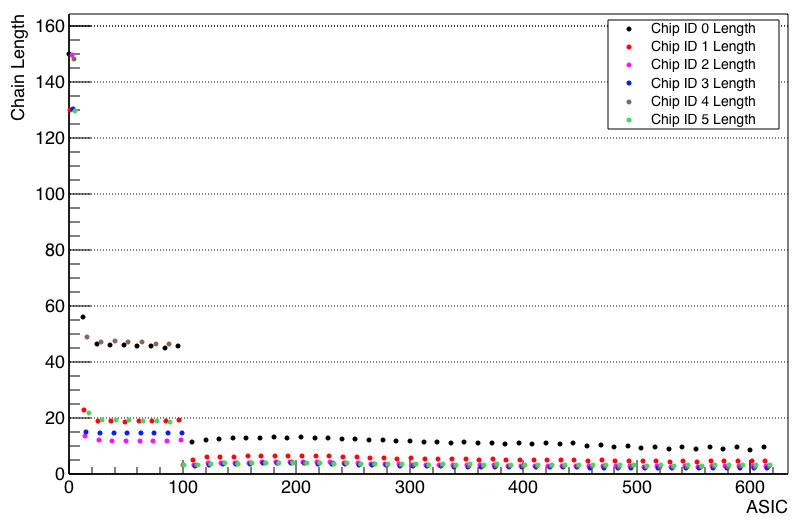
\includegraphics[width=0.75\textwidth]{Mean_ASIC_Graph_Chip}
	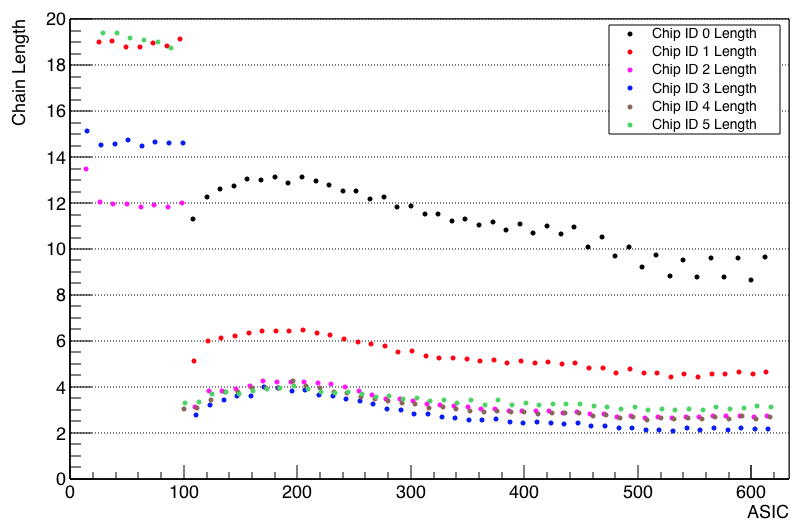
\includegraphics[width=0.75\textwidth]{Mean_ASIC_Graph_Chip_lower_values}
	\caption{The mean data train length for each ASIC, coloured by the chip number.}
\end{figure}

% section event_isolation_flagging_apendix (end)

\end{document}
